%%%%%%%%%%%%%%%%%%%%%%%%%%%%%%%%%%%%%%%%%%%%%%%%%%%%%%%%%%%%%%%%%%%%%%%%%%%%%%%%
\documentclass{article}
\usepackage[a4paper, hmargin={2.8cm, 2.8cm}, vmargin={2.5cm, 2.5cm}]{geometry}
%%%%%%%%%%%%%%%%%%%%%%%%%%%%%%%%%%%%%%%%%%%%%%%%%%%%%%%%%%%%%%%%%%%%%%%%%%%%%%%%

%%%%%%%%%%%%%%%%%%%%%%%%%%%%%%%%%%%%%%%%%%%%%%%%%%%%%%%%%%%%%%%%%%%%%%%%%%%%%%%%
\usepackage[utf8]{inputenc}
\usepackage[T1]{fontenc}
%%%%%%%%%%%%%%%%%%%%%%%%%%%%%%%%%%%%%%%%%%%%%%%%%%%%%%%%%%%%%%%%%%%%%%%%%%%%%%%%


%%%%%%%%%%%%%%%%%%%%%%%%%%%%%%%%%%%%%%%%%%%%%%%%%%%%%%%%%%%%%%%%%%%%%%%%%%%%%%%%
\usepackage{mathtools}
\usepackage{amsthm}
\usepackage{amssymb}
\usepackage{csvsimple}
\usepackage{subcaption}
\usepackage{url}
\usepackage{url}
\usepackage{tikz}
\usepackage{pgfplots}
%%%%%%%%%%%%%%%%%%%%%%%%%%%%%%%%%%%%%%%%%%%%%%%%%%%%%%%%%%%%%%%%%%%%%%%%%%%%%%%%


%%%%%%%%%%%%%%%%%%%%%%%%%%%%%%%%%%%%%%%%%%%%%%%%%%%%%%%%%%%%%%%%%%%%%%%%%%%%%%%%
\usepackage{fancyhdr}
\usepackage{graphicx}
\usepackage{parskip}
\usepackage{listings}
\usepackage{enumitem}
\usepackage{titlesec}
\usepackage[lastpage,user]{zref}
\usepackage{caption}
\usepackage{scrextend}
\usepackage[outputdir=./.latex-out]{minted} % TODO slet hvis du ikke bruger minted
\usepackage{listings}
\usepackage{blindtext}
%%%%%%%%%%%%%%%%%%%%%%%%%%%%%%%%%%%%%%%%%%%%%%%%%%%%%%%%%%%%%%%%%%%%%%%%%%%%%%%%
\newcommand{\python}[1] {
  \mintinline{python}{#1}
}
\newcommand{\tex}[1] {
  \mintinline{latex}{#1}
}
\pagestyle{fancy}
%%%%%%%%%%%%%%%%%%%%%%%%%%%%%%%%%%%%%%%%%%%%%%%%%%%%%%%%%%%%%%%%%%%%%%%%%%%%%%%%
%%%%%%%%%%%%%%%%%%%%%%%%%%%%%%%%%%%%%%%%%%%%%%%%%%%%%%%%%%%%%%%%%%%%%%%%%%%%%%%%
\lhead{\LaTeX webinar} % TODO indsæt venstre sidehoved
\rhead{Study Now} % TODO indsæt højre sidehoved
\cfoot{\thepage\ of \zpageref{LastPage}}
\newtheorem*{prp}{Propostion}
\setlist{nolistsep}
%%%%%%%%%%%%%%%%%%%%%%%%%%%%%%%%%%%%%%%%%%%%%%%%%%%%%%%%%%%%%%%%%%%%%%%%%%%%

%%%%%%%%%%%%%%%%%%%%%%%%%%%%%%%%%%%%%%%%%%%%%%%%%%%%%%%%%%%%%%%%%%%%%%%%%%%%
\title{
  \vspace{13em}
  \large{Study Now} \\
  \Large{\LaTeX webinar} \\
}

\author{
  Benjamin Rotendahl --- Benjamin@Rotendahl.dk
}

\date{
  \vspace{22em}
  \today
}
%%%%%%%%%%%%%%%%%%%%%%%%%%%%%%%%%%%%%%%%%%%%%%%%%%%%%%%%%%%%%%%%%%%%%%%%%%%%
%%%%%%%%%%%%%%%%%%%%%%%%%%%%%%%%%%%%%%%%%%%%%%%%%%%%%%%%%%%%%%%%%%%%%%%%%%%%%%%%

\begin{document}

\clearpage

% Disse linjer skaber forside, evt indholdsfortegnelse, og sætter sidetal
%%%%%%%%%%%%%%%%%%%%%%%%%%%%%%%%%%%%%%%%%%%%%%%%%%%%%%%%%%%%%%%%%%%%%%%%%%%%%
\maketitle		% Forside
\thispagestyle{empty}
\newpage

\thispagestyle{empty}\tableofcontents\newpage % TODO indsæt indholdsfortegnelse eller slet for at fjerne

\setcounter{page}{1}
%%%%%%%%%%%%%%%%%%%%%%%%%%%%%%%%%%%%%%%%%%%%%%%%%%%%%%%%%%%%%%%%%%%%%%%%%%%%%

\section{Introduction}
 Dette dokument fungerer som et \emph{cheatsheet}. Det gennemgår de forskellige
 former for opsætning og funktioner i \LaTeX. Når du selv sidder og skriver, kan
 du enten bruge den færdige PDF som opslagsværk, eller kigge på kildekoden.
 Husk, at du selv kan udvide dokumentet med yderligere sektioner, hvis du finder
 nogle seje funktioner i din videre færd med \LaTeX{}.

\section{\LaTeX{} baggrund}
 Før vi går i gang med syntaksen osv., gennemgår vi, hvordan \LaTeX{} fungerer og
 laver kildekode om til en PDF.
 \LaTeX{} er et skriftsstyringssprog, som bruges til at skrive dokumenter med. Det er
 særligt godt til at skrive dokumenter med matematik, kode og andre
 videnskablige figurer. \LaTeX er en udvidelse af TeX, som blev udgivet af Donald
 Knuth i 1989.

 \subsection{Fra kildekode til PDF}\label{sec:local}
   \LaTeX er ikke et skriveprogam, men et sprog samt compiler\footnote{
     Det, man kalder en \emph{oversætter} på dansk}. Den tager kildekoden, som er skrevet i en
   \emph{editor}, og laver det om til en PDF. En editor til lokalt brug kan
   f.eks. være \emph{Visual studio code}\cite{vscode}. Det er en editor, som kan
   bruges til at skrive alle slags sprog. Man installerer ekstra pakker, som
   udvider dens funktionalitet, f.eks. har den både pakker til at hjælpe med
   python-kode, javascript og \LaTeX{}\cite{latexPackage}.

   Efter koden er skrevet, skal den gives videre til en \emph{compiler}, som
   tager kildekoden og laver det om til en PDF. Det er compileren, som
   inkluderer filer, figuerer osv. Er der en fejl i kildekoden, gør compileren
   sit bedste for at fastslå, hvad fejlen er, og hvordan den kan fixes. Der findes
   forskellige versioner af LaTeX compileren, som prinært varierer i, hvilke
   ekstra pakker og værktøjer de inkulderer.
   ``The latex project TeX''\cite{texLive} har links til distrubtioner for de
   de forskellige styresystemer. Med en compiler og editor installeret er man
   klar til at bygge sit første latex dokument, processen kan ses i
   figuer~\ref{fig:compile}.

   \subsubsection{Overleaf}
     Sektion~\ref{sec:local} forklarer, hvordan du opsætter dit eget miljø lokalt.
     Der findes tjenester som Overleaf\footnote{\url{overleaf.com}}, der fungerer
     på samme måde som google docs. Man arbejder i en webrowser, hvor de giver en et fuldt opsat
     miljø. Man slipper altså for at installere noget lokalt og har nemmere ved
     at dele sit arbejde med eventuelle gruppemedlemmer. Ulempen er, at man ikke
     har samme konfigurationsmuligheder som lokalt, og det kræver internetadgang
     at tilgå.

     \begin{figure}[h]
       \centering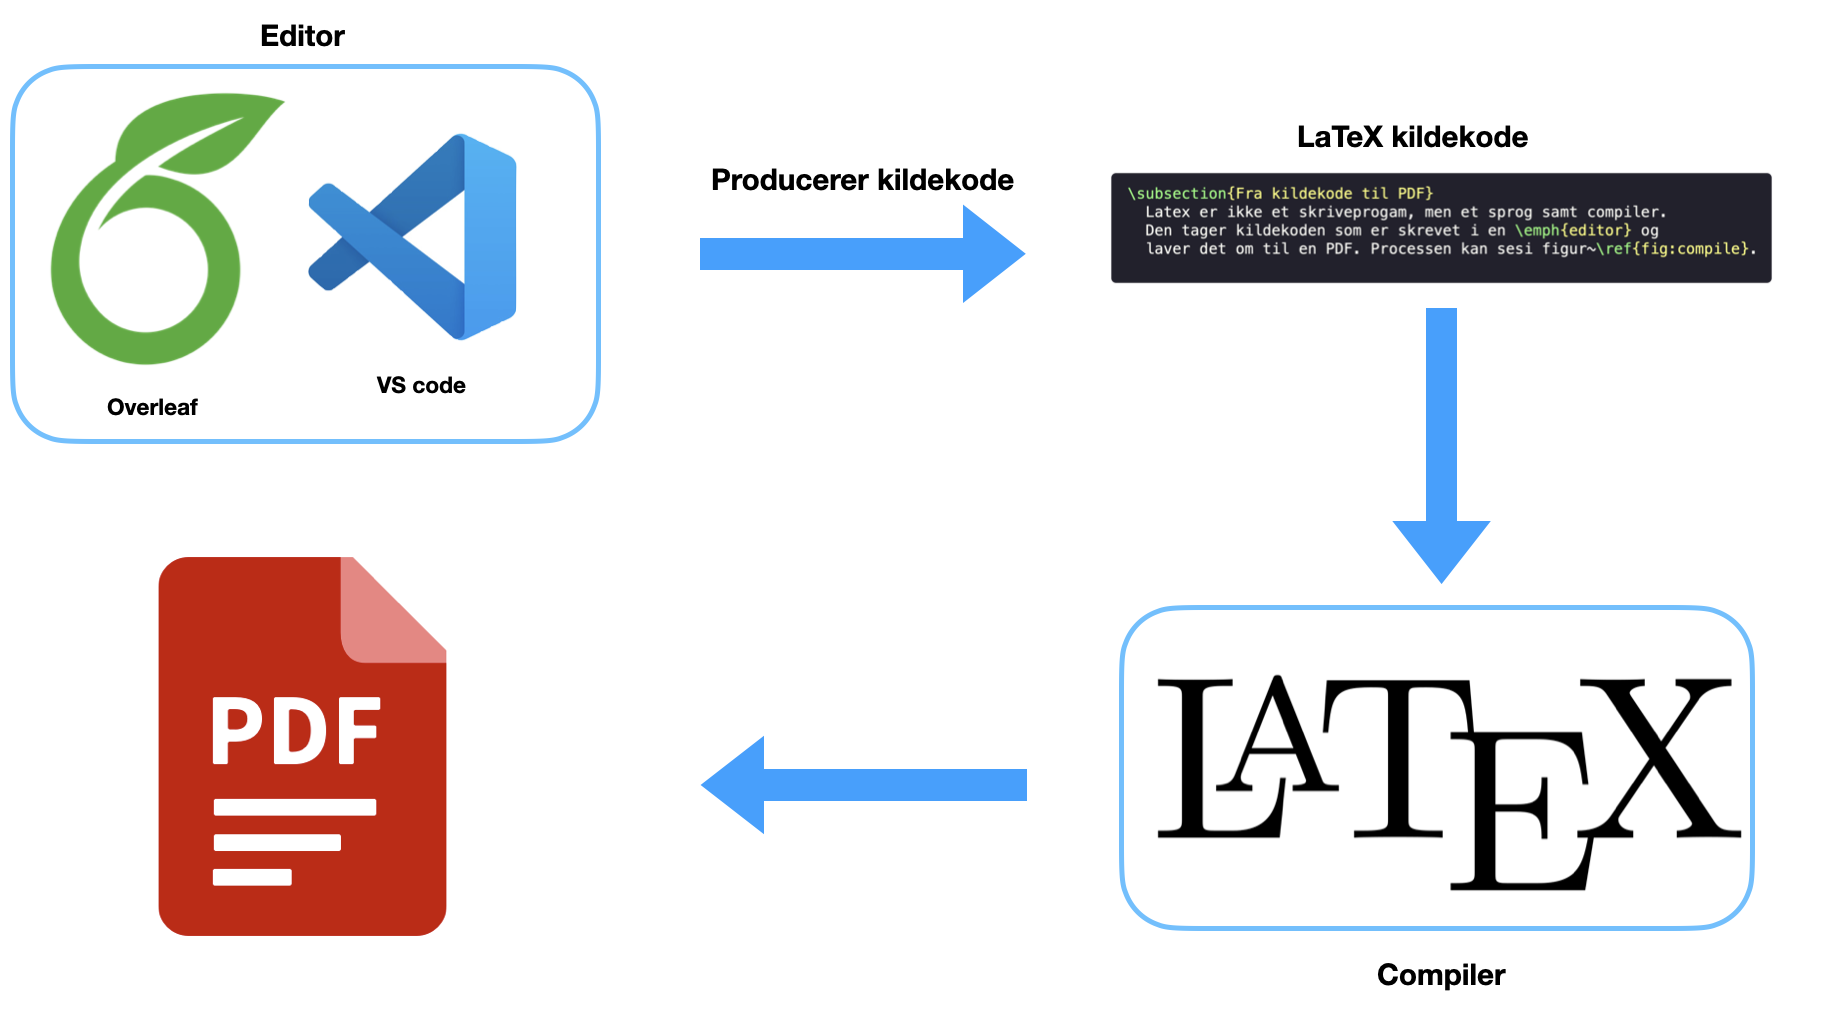
\includegraphics[width=0.9\textwidth]{assets/compile.png}
       \caption{Hvordan man kommer fra kildekode til pdf}\label{fig:compile}
     \end{figure}


 \subsection{\LaTeX{} tankegang \& syntax}
   \LaTeX{} adskiller sig fra programmer som word, google docs, osv. ved ikke at
   være en så såkaldt \emph{WYSIWYG}\footnote{What you see is what you get} editor.
   I stedet for at formattere teksten, mens man skriver, og bruge knapper i det grafiske
   interface til at ændre udseendet, så gør man det via kommandoer. Tanken bagved er, at man
   skal koncenterere sig om sit indhold og lade kompileren om formatteringen via
   kommandoerne.

   En latex-fil består af to dele: den såkaldte \emph{preamble} og dokumentet.
   Preamblen består af kommandoer, som definerer hvilken type dokument, vi
   arbejder med, laver global opsætning og inkluderer de pakker, dokumenetet
   kræver.

   \subsubsection{Kommando syntax}
     En kommando består af en ``backslash'' efterfulgt af et kommandonavn.
     Tager kommandoen parametre, skal de skrives i krølleparanteser
     efter. F.eks. kan vi skrive \LaTeX{} ved at skrive \tex{\LaTeX}. Der findes
     genveje til de mest gængse kommandoer.
     \begin{description}
       \item[Linjeskift] \LaTeX{} sørger selv for at lave linjeskift i ens tekst.
         Laver man et manuelt linjeskift, ignorer programmet det. Det er på den måde, at man har
         bedre mulighed for selv at formattere ens kildekode, uden det påvirker den
         endelige pdf. Ønsker man selv at bestemme et linjeskift, kan man enten indsætte to
         linjeskift i sin egen kode, skrive \tex{\linebreak} eller to backslashes.
         \tex{\\}

       \item[Tvunget mellemrum] Ligesom med linjeskift, fjerner \LaTeX{} også
         nogle mellemrum. Hvis man har man sat flere end et, bliver de slået sammen til et enkelt.
         Ønsker man et tvunget mellemrum, skriver man \tex{hej ~~~ verden}

       \item[Ny side] Ønsker man at tvinge \LaTeX til at skifte til en ny side,
         skriver man \tex{\newpage}

       \item[Anførselstagn] Ønsker man at sætte tekst i ``anførselstegn'', gøres
         det ved at skrive \tex{``anførselstegn''}

       \item[Kommentar] Ønsker man at inkuldere noget tekst i sin kildekode, men
         ikke i den færdige pdf, kan man lave en \emph{Kommentar}. Det er brugbart
         for at lave påmindelser til sig selv eller gruppemedlemmer. Sætter man
         et \(\%\) tegn, vil resten af linjen ikke blive inkluderet. For at
         skrive \(\%\), sætter man så en backslash foran \tex{\%}


       \item[Matematik] Der findes to måder at skrive matematik på, den ene er
         \emph{inline}, hvor matematikken står inde i teksten, f.eks. \(x^2 +4\),
         hvilket gøres ved at skrive \tex{\(x^2 +4\)}. Den anden er \emph{display}
         mode, hvor matematikken står udenfor teksten, det skrives sådan her:
         \tex{\[x^2 +4\]}. f.eks \[x^2 +4\]
       \item[Miljøer] Ved større kommandoer kan det blive svært at skrive det
         hele i krølleparanterser bagefter. Til sådane kommandoer kan man skrive det
         med miljønotation. Ønkser vi f.eks. at have en linje i midten, kunne
         vi skrive
         \tex{\centering{\\ Jeg er i midten \\}}.
         \centering{\\ Jeg er i midten \\}
         Var min tekst længere, ville det være nemmere at skrive

         Der findes mange miløjer til at lave alt fra lister, matricer, tabeller,
         figurer osv.

     \end{description}

     Listing~\ref{lst:latex} viser en simpel latex-fil, hvor de overstående
     \LaTeX{} kommandoer bliver brugt til at lave en simpel pdf.
     \begin{listing}[!h]
       \begin{minted}[tabsize=1]{latex}
				\documentclass{article}
				\usepackage{amsmath} % pakke til ekstra matematiksymboler
				\usepackage{graphicx} % pakke til figurer og billeder

				\title{
					\large{Study Now} \\
					\Large{\LaTeX webinar} \\
				}

				\author{
					Benjamin Rotendahl --- Benjamin@Rotendahl.dk
				}

				\begin{document}
						\maketitle
						\section{Introduction}
							Dette dokument viser hvordan \(\dots\)
				\end{document}
   		\end{minted}
       \caption{Ekspempel på simplet latex dokument}\label{lst:latex}
     \end{listing}

 \subsection{Referencemateriale og problemløsning}
   At lære \LaTeX er en løbende proces. Efter at have lært det basale, skal man
   bare i gang med at skrive. Der er for mange kommandoer til at sætte sig ned
   og lære det hele på en gang. En bedre proces er at kaste sig ud i det og
   løse problemer og lære nye kommandoer undervejs. Hvis man f.eks. ønsker at
   inkludere to figurer ved siden af hinanden og ikke ved det endnu, er google
   den bedste løsning. Sådan en søgning vil typisk give et eksmpel fra
   \emph{tex.stackexchange.com} eller ligende, og her kan man så kopiere eksemplet
   fra. Ønsker man en større guide, findes der ``The Not So Short Introduction to
   \LaTeX\footnote{http://web.math.ku.dk/~holm/download/lshort.pdf}'', som
   går mere i dybden med \LaTeX.

   Når man laver fejl i sin latex-kode, kan ens dokument ikke kompileres, og der
   vil ikke blive lavet en pdf. Compileren laver en log, hvori den prøver at
   beskrive, hvorfor den fejlede. Det er lidt en kunst at læse de logs og finde
   ud af, hvad der egentlig er i vejen. Skriver vi f.eks. \tex{\newpge} i stedet
   for \tex{\newpage}, giver loggen os følgende linjer begravet i omkring 300 linjer.
   \begin{verbatim}
		/Users/rotendahl/Documents/projects/study_now/latex/cheetsheet.tex:241: Undefined control sequence.
		l.241 ...ewpage} vi f.eks \newpge
	 \end{verbatim}
   Den fortæller os, hvilken linje der fejlde, og at det sker, fordi den ikke ved,
   hvad \tex{\newpge} betyder. Når man først har lært at lede i loggen efter det
   vigtige, kan man hurtigt fixe sine fejl eller google log-beskeden og lære,
   hvorfor den gik i stykker.



\section{Matematik i \LaTeX}
 Latex' største styrke er dens evne til at formatere matematisk notation.
 For at skrive matematik skal man fortælle compileren, at den skal gå i
 \emph{math mode} for så at kunne skrive matematik specifikke kommandoer.
 Prøver man f.eks. at skrive \tex{\pi} uden at være i math mode, fejler den.
 Man kan som nævnt gå i inline math mode ved at skrive \tex{\(\pi\)}, som giver
 \(\pi\). Der findes også miljøer, som sætter en i math mode, f.eks. \tex{\equation}
 miløjet. Det går det også muligt at lave referencer til sine formler, f.eks.
 viser ligningen \eqref{dot} formlen for prikproduktet af to vectorer.
 \begin{equation}\label{dot}
   \vec{a} \cdot \vec{b} = \sum_{i=1}^{n} a_i b_i
 \end{equation}
 Koden, der producerer overstående, kan ses i ekspempel~\ref{lst:dot}
 \begin{listing}[!h]
   \begin{minted}[tabsize=1]{latex}
		\begin{equation}\label{dot} % Label som kan bruges som reference
			\vec{a} \cdot \vec{b} = \sum_{i=1}^{n} a_i b_i
		\end{equation}
	\end{minted}
   \caption{Ligning for prikproduktet}\label{lst:dot}
 \end{listing}

 Ønsker vi at have en flere trin i en udledning, kan vi bruge flalign-miløjet.
 Der kan man have flere linjer, som bliver centreret efter placeringen af \tex{&}
 symbolet.
 \begin{flalign}
   f(x, y)                       & = 3x^2y + y^2 \\
   \frac{\partial f}{\partial x} & = 6xy         \\
   \frac{\partial f}{\partial y} & = 3x^2 + 2y
 \end{flalign}
 Koden, der skaber overstående, kan ses i listing~\ref{lst:diff}. Ønsker man at
 fjerne tallene ude i højre side, kan det gøres ved at erstatte \tex{flaling} med
 \tex{flaling*}.
 \begin{listing}[!h]
   \begin{minted}[tabsize=1]{latex}
		\begin{flalign}
			f(x, y)                       & = 3x^2y + y^2 \\
			\frac{\partial f}{\partial x} & = 6xy         \\
			\frac{\partial f}{\partial y} & = 3x^2 + 2y
		\end{flalign}
 \end{minted}
   \caption{Eksempel på formler centreret over flere linjer}\label{lst:diff}
 \end{listing}

 For at lave paranteser i sine formler skal man bare skrive som normalt, men
 ønsker man, at de skalerer efter indholdet, så kræver det, at man skriver
 \tex{\left ( x^2 \right )} rundt om. Typen af parenteser efter \tex{\left, \right}
 kommandoen bestemmer, hvordan det ser ud. Listing~\ref{lst:par} viser, hvordan følgende
 er lavet.
 \begin{flalign*}
   f(x) & = (\frac{1}{x})^2                              \\ % Ikke skaleret parantes
   f(x) & = \left ( \frac{1}{x} \right )^2               \\ % skaleret parantes
   x    & \in \left [ \frac{1}{4},  \frac{1}{2} \right ] \\ % Firkanten paranteser
   x    & \in \left
   \{\frac{1}{n}, \frac{2}{n}, \frac{3}{n}, \dots, \frac{n}{n} \right \} % krølle paranteser
 \end{flalign*}

 \subsection{Matematikoperationer og notationer}
   Følgende er et opslagsværk med de mest gængse matematikoperationer og notationer.
   Først er der en liste over syntaxen, som bliver efterfulgt af et eksemplet på, hvordan det
   bliver formateret, og til sidst står koden for eksemplet. Eksemplerne i listen antager,
   at man allerede er i math mode, f.eks. \tex{\begin{flalign} x + 1 \end{flalign}}
   eller f.eks. i display mode \tex{\[ x + 1 \]}
   \begin{description}
     \item[Standardoperationer] for at skrive \(+, -\) gør man bare som normalt.
       Ønsker man et gangetegn kan det gøres med enten \tex{a \cdot b, a \times b},
       som bliver til \(a \cdot b, a \times b\)
       \[
         1+1 -y \cdot x
       \]
     \item[Brøker] for at lave en brøk bruger man \tex{\frac{a}{b}} kommandoen.
       Indholdet af den første krølleparantes sættes i tælleren og, indholdet af
       den næste sættes i nævneren. Man kan også have brøker i brøker.
       \[
         \frac{a}{b} + \frac{a}{\frac{b}{c}}
       \]
     \item[Potenser og subscript] Ønsker man at skrive f.eks. \(x^2, x_i\), gøres
       det ved at skrive \tex{\(x^2, x_i\)}. Vil man have mere end et tegn inkluderet,
       skal det sættes i krølleparenteser, f.eks. \tex{\(x_{i+1}\)}, som bliver til
       \(x_{i+1}\).

     \item[Sum og integraler] Ønsker vi at lave et summationstegn, kan det
       gøres ved at skrive sum-kommandoen efterfulgt af en øvre og nedre potens.
       \tex{\sum_{i=1}^{n} a_i b_i} eller \tex{\int_{i=1}^{n} a_i b_i}
       Et integrale kan skrives på samme måde, men med \emph{int} i stedet for
       \tex{\int{i=1}^{n} a_i b_i}
       \[
         \sum_{i=1}^{n} a_i b_i + \int_{i=1}^{n} x
       \]

   \end{description}




   \begin{listing}[!h]
     \begin{minted}[tabsize=1]{latex}
	 \begin{flalign*}
		 f(x) &= (\frac{1}{x})^2  \\ % Ikke-skaleret parantes
		 f(x) &= \left ( \frac{1}{x} \right )^2  \\ % skaleret parantes
		 x  \in \left [ \frac{1}{4},  \frac{1}{2} \right ] \\ % Firkantede paranteser
		 x  \in \left \{\frac{1}{n}, \frac{2}{n}, \frac{3}{n}, \dots, \frac{n}{n} \right \} % krølleparanteser
	 \end{flalign*}
\end{minted}
     \caption{Eksempel på forskellige typer paranteser}\label{lst:par}
   \end{listing}

 \subsection{Matricer og vektorer}
   Latex gør det nemt at skrive matricer og vektorer. Det gøres med miljøkommandoerne \\
   \tex{\pmatrix, \bmatrix, \bMatrix}, som laver en matrice med henholsvis
   \( (, [, \{ \). Inde i milljøet skriver man elementerne i hver række adskilt af
   \tex{&}, og rækkerne adskilles enkeltvis af \tex{\\}. Eksemplet herunder kan findes i listing
   ~\ref{lst:matrix}. Læg mærke til, at kommandoen \tex{\quad} bruges til at lave
   afstand mellem matricerne, og hvordan \tex{\dots, \vdots, \ddots} bruges til at
   lave den sidste matrice.
   \[
     \begin{pmatrix}
       1 & 2 & 3 \\
       4 & 5 & 6 \\
       7 & 8 & 9
     \end{pmatrix}
     ,\quad
     \begin{bmatrix}
       1 & 2 & 3 \\
       4 & 5 & 6 \\
       7 & 8 & 9
     \end{bmatrix}
     ,\quad
     \begin{Bmatrix}
       1 & 2 & 3 \\
       4 & 5 & 6 \\
       7 & 8 & 9
     \end{Bmatrix}
     ,\quad
     \begin{bmatrix}
       1      & \dots  & n      \\
       \vdots & \ddots & \vdots \\
       n      & \dots  & n
     \end{bmatrix}
   \]
   \begin{listing}[!h]
     \begin{minted}[tabsize=1]{latex}
			\[
				\begin{pmatrix}
					1 & 2 & 3 \\
					4 & 5 & 6 \\
					7 & 8 & 9
				\end{pmatrix}
				,\quad
				\begin{bmatrix}
					1 & 2 & 3 \\
					4 & 5 & 6 \\
					7 & 8 & 9
				\end{bmatrix}
				,\quad
				\begin{Bmatrix}
					1 & 2 & 3 \\
					4 & 5 & 6 \\
					7 & 8 & 9
				\end{Bmatrix},
				,\quad
				\begin{bmatrix}
					1      & \dots  & n      \\
					\vdots & \ddots & \vdots \\
					n      & \dots  & n
				\end{bmatrix}
			\]
 \end{minted}
     \caption{Eksempel på forskellige typer matricer}\label{lst:matrix}
   \end{listing}


\section{Figurerer}
 Latex understøtter også figuerer, som er lavet med \tex{figure} miljøet.
 En figur er en såkaldt \emph{float}, det vil sige, at \LaTeX selv finder ud af
 at indsætte indholdet et sted på siden. En figur kan indeholde tekst, tabeller,
 billeder, osv. At lave figur gøres typisk ved:
 \begin{listing}[!h]
   \begin{minted}[tabsize=1]{latex}
			\begin{figure}[h]
				\centering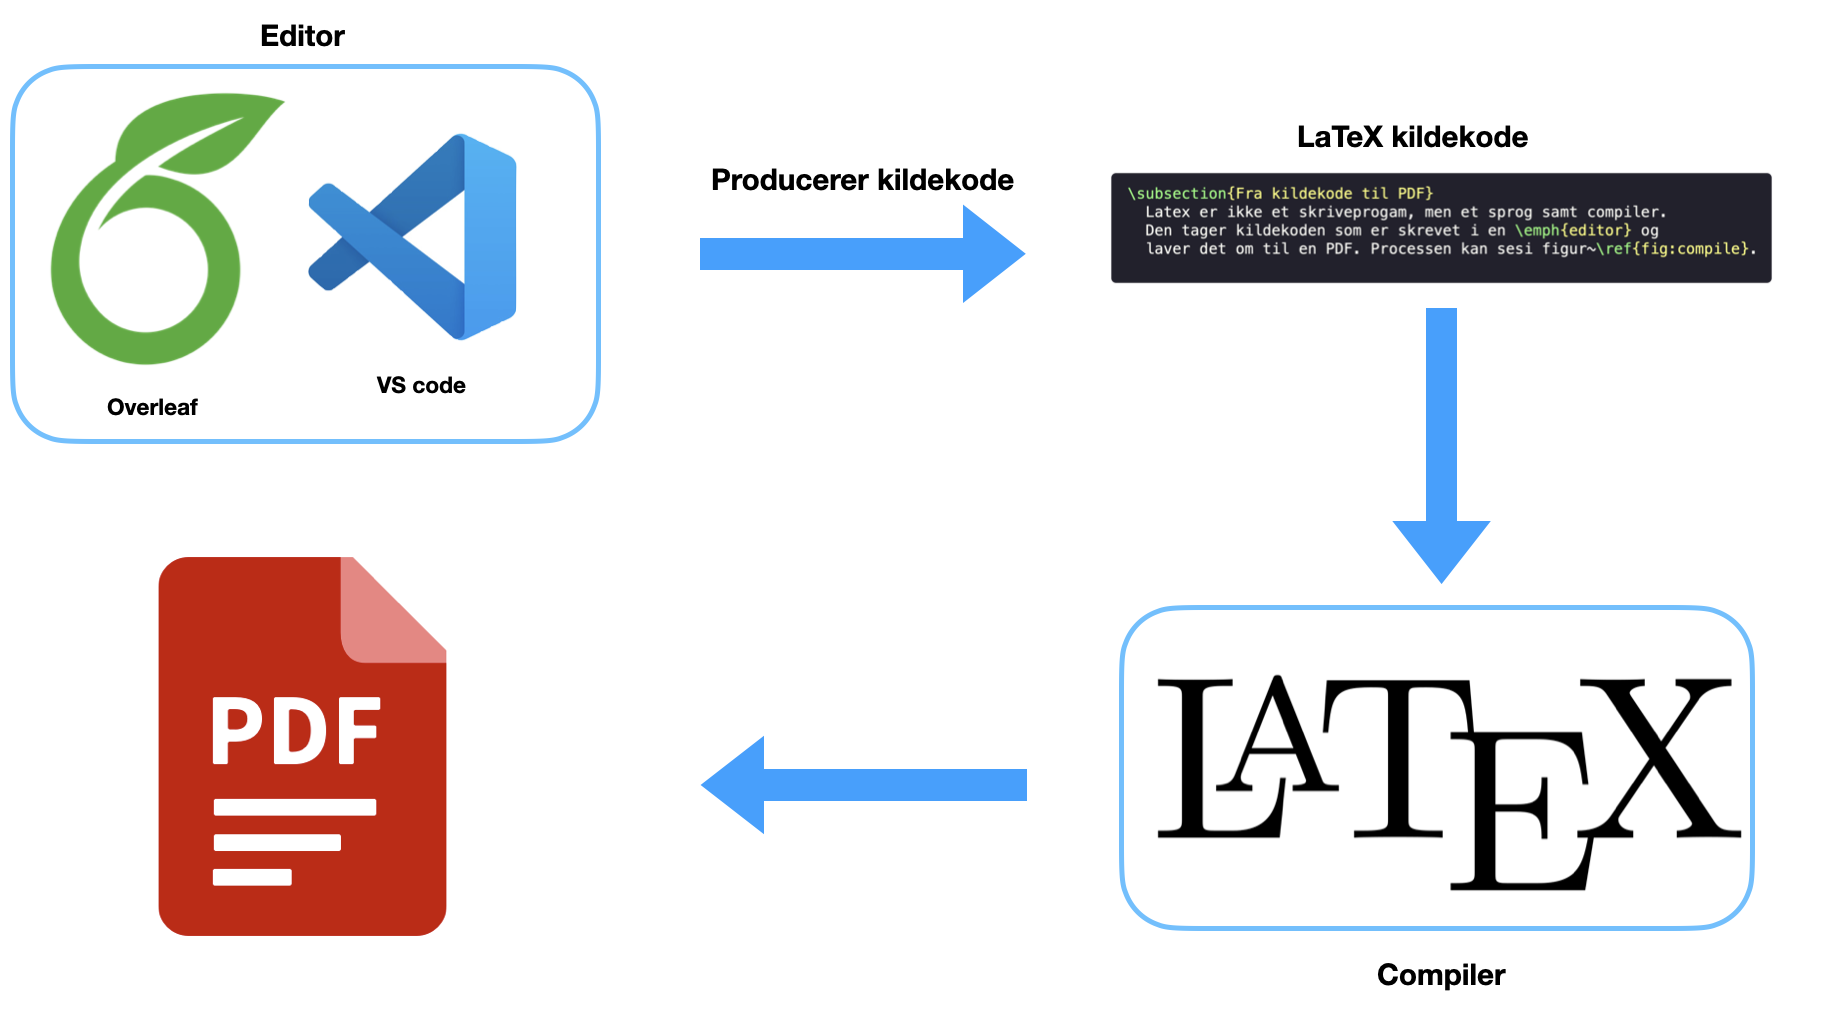
\includegraphics[width=0.9\textwidth]{assets/compile.png}
				\caption{Hvordan man kommer fra kildekode til pdf}\label{fig:compile}
			\end{figure}
		\end{minted}
   \caption{Eksempel på indsættlese af figur}\label{lst:matrix}
 \end{listing}
 I overstående starter vi først et figurmiljø. På første linje betyder \tex{[h]},
 at figueren skal være \emph{here}, som fortæller latex, at vi prioriterer, at
 figueren er så tæt på naboteksten som muligt. Sætter vi en af \tex{[t], [b]}
 ind i stedet, vil compileren enten sætte det i toppen eller bunden af siden.
 Vi bruger \tex{\centering} til at sætte vores billede i midten af siden,
 \tex{\includegraphics} indsætter billedet og \tex{\width=.9} sætter billedets
 bredde til \(90\%\) af sidens bredde. Den sidste del af \tex{\includegraphics}
 kommandoer skal være i krølleparanteser og er stien til den fil, der skal inkluderes.
 Ved at bruge \tex{\caption} og \tex{\label} vil vi få et label til vores figur
 og en figurbeskrivelse.
 \subsection{TikZ}
   Man kan bruge udvidelsen TikZ til at lave grafer, plots, og andre figurer.
   TiKZ kan være rigtig smart, men det kræver en god del at lære hvordan man
   bruger det. Alternativt kan man fint lave sine grafer i python, excel eller
   andet og importere dem som billeder. Figur~\ref{fig:tikz} viser et plot lavet
   i TikZ and eksempel ~\ref{lst:tikz} viser koden bag.
   \begin{figure}[h]
     \centering
     \begin{tikzpicture}
       \begin{axis}[xmin=-10,xmax=10,ymin=-20,ymax=20, samples=100]
         \addplot[blue, thick] (x,5*x^3+3*x);
         \addplot[red, thin] (x*x,x);
       \end{axis}
     \end{tikzpicture}
     \caption{Eksempel på en tikz figur}\label{fig:tikz}
   \end{figure}
   \begin{listing}[!h]
     \begin{minted}[tabsize=1]{latex}
    \begin{figure}
     \centering
     \begin{tikzpicture}
      \begin{axis}[xmax=9,ymax=9, samples=50]
      \addplot[blue, thick] (x,5*x^2+3*x);
      \addplot[red, thin] (x*x,x);
    \end{axis}
  \end{tikzpicture}
 \caption{Example of a tikz graph}\label{tiks:graph}
\end{figure}
  \end{minted}
     \caption{Example creating a figure in tikz}\label{lst:tikz}
   \end{listing}


\section{Lister}
 I latex bruger man primært tre typer miljøer til lister. Alle typer skrives
 med et \\
 \tex{\begin{liste_type} \item ting 1 \item ting 2 \end{liste_type}}.\\
 Alle listetyper kan indeholde lister, Latex sørger selv for, at listerne formateres
 korrekt. Koden, der laver listerne herunder, kan ses i listing~\ref{lst:list}
 \begin{description}
   \item[\tex{itemize}] En punktliste med prikker for at markere listeenheder
     \begin{itemize}
       \item Et punkt
       \item Et andet punkt
       \item Punkt med underliste  \begin{itemize}
               \item Et underlistepunkt
               \item Et andet underlistepunkt
             \end{itemize}
     \end{itemize}
   \item[Enumerate] En liste med tal for at markere listeenheder. Tallene bliver automatisk
     indsat. Man kan enda have en Enumerate inde i en Enumerate, hvor den selv ændrer tæller.
     \begin{enumerate}
       \item Et punkt
       \item Et andet punkt
       \item Punkt med underliste \begin{enumerate}
               \item Et underlistepunkt
               \item Et andet underlistepunkt
             \end{enumerate}
     \end{enumerate}
   \item[\tex{description}] En liste med en beskrivelse af listepunkter, ud for
     hvert item skal der være en punktbeskrivelse \tex{\item[beskrivelse]}
     \begin{description}
       \item[det første] Et punkt
       \item[det andet] Et andet punkt
       \item[det trejde] Punkt med underliste \begin{description}
           \item[første underpunkt] Et underlistepunkt
           \item[andet underpunkt] Et andet underlistepunkt
         \end{description}
     \end{description}
 \end{description}
 \begin{listing}[!h]
   \begin{minted}[tabsize=1]{latex}
		\begin{itemize}
			\item Et punkt
			\item Et andet punkt
			\item Punkt med underliste  \begin{itemize}
							\item Et underlistepunkt
							\item Et andet underlistepunkt
						\end{itemize}
		\end{itemize}

		\begin{enumerate}
			\item Et punkt
			\item Et andet punkt
			\item Punkt med underliste \begin{enumerate}
							\item Et underlistepunkt
							\item Et andet underlistepunkt
						\end{enumerate}
		\end{enumerate}

		\begin{description}
			\item[det første] Et punkt
			\item[det andet] Et andet punkt
			\item[det trejde] Punkt med underliste \begin{description}
					\item[første underpunkt] Et underlistepunkt
					\item[andet underpunkt] Et andet underlistepunkt
				\end{description}
		\end{description}
\end{description}
	 \end{minted}
   \caption{Forskellige typer af lister. }\label{lst:list}
 \end{listing}



\section{Tabeller}
 For at lave tabeller bruger man de to miljøer \tex{\table, \tabular}, der fungerer
 som \tex{\figure, \includegraphics}. Tabel~\ref{table:data} er lavet med koden i
 listing~\ref{lst:table}. Vi starter ligesom i figure med at skrive \tex{[h]} for
 at markere, at tabellen skal være her. \tex{\centering} sætter tabellen i midten af
 dens \emph{float}. Miljøet \tex{\tabular} starter tabellen, i krølleparentersene, der står
 bagefter, fortæller vi kompileren hvor mange rækker, vores tabel fylder, og hvordan
 de skal adskilldes med \(|\) symbolet. Skrev vi \tex{\tabular}{|l|c r|}, vil
 tabellen have tre søjler, hvor teksten i den første står til venstre, i miden
 vil teksten være centreret, og den sidste vil stå til højre. Der vil også kun
 være en skillelinje mellem de to første søjler.
 I tabellen skriver vi elementerne ligesom i en matrice. Vi bruger \tex{&} for at
 adskille elementer og \tex{\\} for at adskille rækker. Vi kan bruge \tex{\hline}
 til at lave en skillelinje mellem rækkerne.
 \begin{table}[h]
   \centering
   \begin{tabular}{||c c | c c||}
     \hline
     søjle1 & søjle2 & søjle4 & søjle4 \\  \hline
     1      & 6      & 87837  & 787    \\
     2      & 7      & 78     & 5415   \\
     3      & 545    & 778    & 7507   \\
     4      & 545    & 18744  & 7560   \\
     5      & 88     & 788    & 6344   \\
     \hline
   \end{tabular}
   \caption{Eksempel på manuelt skrevet tabel}\label{table:data}
 \end{table}
 \begin{listing}[!h]
   \begin{minted}[tabsize=1]{latex}
	  \begin{table}[h]
			\centering
			\begin{tabular}{||c c | c c||}
				\hline
				søjle1 & søjle2 & søjle4 & søjle4 \\  \hline
				1      & 6      & 87837  & 787    \\
				2      & 7      & 78     & 5415   \\
				3      & 545    & 778    & 7507   \\
				4      & 545    & 18744  & 7560   \\
				5      & 88     & 788    & 6344   \\
				\hline
			\end{tabular}
			\caption{Eksempel på manuelt skrevet tabel}\label{table:data}
		\end{table}
	\end{minted}
   \caption{Eksempel på tabel }\label{lst:data}
 \end{listing}
 \subsection{Automatiske tabeller}
   Har man en tabel i csv-form, f.eks. fra python eller excel, kan den inkluderes
   ved at sætte pakken \tex{\usepackage{csvsimple}} i sin preamble.
   \begin{table}[h]
     \centering\csvautotabular{assets/dices.csv}
     \caption{Automatic table from csc}\label{table:dices}
   \end{table}
   Det kan gøres ved at skrive:
   \begin{listing}[!h]
     \begin{minted}[tabsize=1]{latex}
     \begin{table}[h]
       \centering\csvautotabular{assets/dices.csv}
       \caption{Automatic table from csc}\label{table:dices}
     \end{table}
     \caption{Eksempel på automatisk tabel }\label{lst:dices}
		\end{minted}
     \caption{Code to generate automatic listing}\label{lst:dices}
   \end{listing}


\section{Kodetekst}
 For at inkludere f.eks. pyton-kode i sit program kan det også enten gøres
 manuelt eller automatisk fra en fil. Ønkser vi f.eks. at inkludere en bid
 python i vores kode som vist i tabel:
 \begin{listing}[!h]
   \begin{lstlisting}[language=python, tabsize=1]
			def fib(x):
				if x == 1 or x == 2:
					return 1
				else:
					return fib(x-1) + fib(x-2)
			\end{lstlisting}
 \end{listing}
 Koden kan ses her:
 \begin{listing}[!h]
   \begin{minted}[tabsize=1]{latex}
		\begin{listing}[!h]
			\begin{lstlisting}[language=python, tabsize=1]
				 def fib(x):
					 if x == 1 or x == 2:
						 return 1
					 else:
						 return fib(x-1) + fib(x-2)
				 \end{lstlisting}
	\caption{Eksempel på automatisk tabel }\label{lst:dices}
 \end{minted}
   \caption{Code to generate automatic listing}\label{lst:dices}
 \end{listing}

 Ønkser man at læse kode fra en fil eller få bedre syntax highligting som
 ved eksemplernen på \LaTeX i dette dokument, skal man bruge pakken \emph{minted}.
 Det kræver en python-installation på systemet. Følg guiden på deres github:
 \url{https://github.com/gpoore/minted}

\section{Referencer}
 I ens latex-kode kan man referre til sine egen figurer og tabeller ved at
 skrive \tex{~\ref{ref:name}}, hvor \emph{ref:name} er det, man har skrevet i dens label.
 Man kan bruge labels til sektioner, tabeller, figuerer og lignigner.
 Udover interne referencer kan man lave en bibliograpfifil, som indeholder referencer
 til videnskablige arktiler, hjemmesider, bøger, osv.
 En bibliograpfifil kan f.eks. hedde \emph{references.bib} og have indhold som
 vist i listing~\ref{lst:big}
 \begin{listing}[!h]
   \begin{minted}[tabsize=1]{bibtex}
		@article{attention,
		author    = {Vaswani, Ashish and Shazeer, Noam and Parmar, Niki and Uszkoreit},
		eprint    = {1706.03762},
		journal   = {arXiv},
		keywords  = {Language Transformer},
		rating    = {5},
		title     = {{Attention Is All You Need}},
		year      = {2017}
	}

	@misc{latexPackage,
		howpublished = {\url{
			https://marketplace.visualstudio.com/items?itemName=James-Yu.latex-workshop
		}},
		title        = {VS Code Latex Package}
	}
	@misc{texLive,
		howpublished = {\url{https://www.latex-project.org/get/}},
		title        = {The LaTex Project}
	}
	@misc{vscode,
		howpublished = {\url{https://code.visualstudio.com}},
		title        = {Microsoft Visual Studio Code}
	}
\end{minted}
   \caption{Code to generate automatic listing}\label{lst:dices}
 \end{listing}
 Når den fil er lavet kan man inkludere den i sin latex via:
 \begin{listing}[!h]
   \begin{minted}[tabsize=1]{latex}
		\bibliography{assets/references}{}
		\bibliographystyle{plain}
\end{minted}
   \caption{Code to generate automatic listing}\label{lst:dices}
 \end{listing}
 Ønsker jeg så at referere til artiklen med titlen
 \emph{Attention Is All You Need}\cite{attention} skriver man
 \tex{\cite{attention}}.



 \newpage
 \appendix
 \bibliography{assets/references}{}
 \bibliographystyle{plain}


\end{document}
